\chapter{Pengenalan Cloud Computing dan Infrastruktur Pengembangan Aplikasi Berbasis Node.js}

\section{Apa itu Cloud Computing?}

Cloud Computing, \index{Cloud Computing} atau sering diterjemahkan sebagai ``Komputasi Awan'' dalam bahasa Indonesia mempunyai berbagai definisi:\index{Cloud Computing!Definisi}
\begin{itemize}
  \item \textbf{Wikipedia}: penggunaan sumber daya komputasi (peranti keras dan peranti lunak) yang berfungsi untuk memberikan layanan melalui suatu jaringan (pada umumnya Internet)\footnote{\url{http://en.wikipedia.org/wiki/Cloud_computing}}.
  \item \textbf{NIST\footnote{The National Institute of Standards and Technology}}: model yang memungkinkan akses jaringan ubiquitous (dari mana saja), nyaman, on-demand (saat ada permintaan) ke sekumpulan sumber daya komputasi yang dikonfigurasi untuk berbagi (jaringan, server, penyimpanan, dan berbagai layanan lain) yang dapat dengan cepat ditetapkan dan dirilis dengan usaha yang minimal dari manajemen ataupun interaksi dengan penyedia layanan\footnote{\url{http://csrc.nist.gov/publications/PubsSPs.html\#800-145}}.
\end{itemize}

Jika diwujudkan secara visual, Cloud Computing bisa dilihat pada Gambar~\ref{fig:ccsam}\footnote{Gambar dibuat oleh Sam Johnston, diambil dari \url{http://en.wikipedia.org/w/index.php?title=File:Cloud_computing.svg&page=1}}

  \begin{figure}[t]
    \begin{center}
      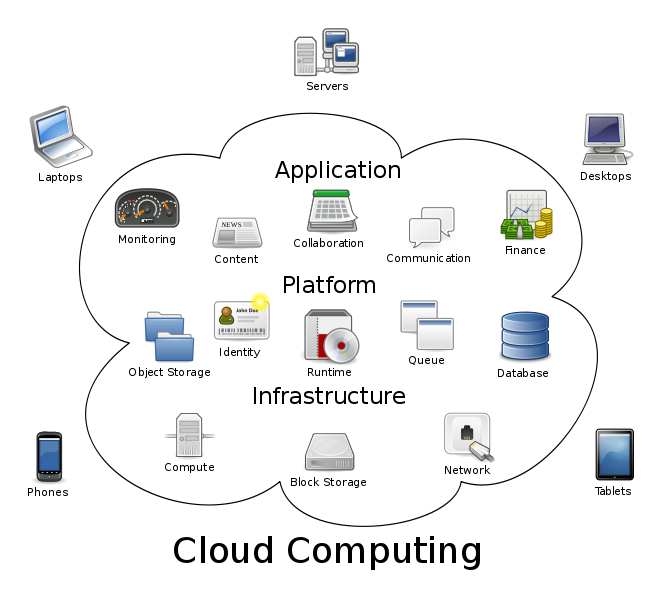
\includegraphics[scale=0.5]{images/662px-Cloud_computing.png}
    \end{center}
    \caption{Model Cloud Computing}
    \label{fig:ccsam}
  \end{figure}

\section{Karakteristik Cloud Computing}

Menurut NIST, ada beberapa karakteristik dari Cloud Computing:\index{Cloud Computing!Karakteristik}
\begin{itemize}
  \item \textbf{On-demand self-service}: layanan bisa diperoleh pada saat diminta, tanpa intervensi atau interaksi manusia di sisi penyedia jasa. 
  \item \textbf{Broad network access}: tersedia melalui jaringan dengan berbagai peranti yang umum (komputer, tablet, HP, dan lain-lain)
  \item \textbf{Resource pooling}: sumber daya komputasi dari penyedia jasa terkumpul untuk melayani.
  \item \textbf{Rapid elasticity}: skalabilitas.
  \item \textbf{Measured service}: penggunaan sumber daya bisa diukur, di-monitor, dikendalikan, dan dilaporkan.
\end{itemize}

Karakteristik lain yang tidak kalah penting adalah \textit{multitenancy}. \textit{Multitenancy} merupakan suatu prinsip dalam arsitektur software. Pada arsitektur tersebut, satu instan dari software berjalan pada server, melayani banyak organisasi klien. Aplikasi dirancang untuk mempartisi data dan konfigurasinya secara virtual dan setiap organisasi klien tersebut bekerja dengan instan aplikasi virtual tersebut\footnote{\url{http://en.wikipedia.org/wiki/Multitenancy}}. \index{Multitenancy}

\section{\textit{Public} dan \textit{Private} Cloud Computing}

\index{Cloud Computing!Private}Cloud Computing bisa dibangun untuk keperluan pribadi suatu organisasi dan (secara legal) hanya bisa diakses oleh organisasi yang bersangkutan. Tipe tersebut dikenal dengan \textit{Private Cloud Computing}. \index{Cloud Computing!Public}Sementara itu, jika sumber daya Cloud Computing bisa diakses oleh publik (dengan hak akses yang sesuai), maka model tersebut dikenal sebagai \textit{Public Cloud Computing}. Pembahasan di buku ini adalah pembahasan tentang \textit{Public Cloud Computing} dan semua referensi tentang Cloud Computing di buku ini akan menunjuk pada \textit{Public Cloud Computing} kecuali dinyatakan lain.

\section{Model Layanan Cloud Computing}

\index{Cloud Computing!Model layanan}Model layanan pada Cloud Computing akan berkembang sesuai kebutuhan konsumen serta inovasi dari berbagai penyedia layanan. Saat ini, pada umumnya, ada tiga model layanan:
\begin{itemize}
  \item \textbf{SaaS} (\textit{Software as a Service}): layanan berupa aplikasi yang ditempatkan pada infrastruktur penyedia layanan, siap digunakan oleh konsumen.
  \item \textbf{PaaS} (\textit{Platform as a Service}): menyediakan layanan ke konsumen berupa platform untuk men-deploy aplikasi.
  \item \textbf{IaaS} (\textit{Infrastructure as a Service}): menyediakan layanan ke konsumen berupa berbagai sumber daya komputasi (pemrosesam, penyimpanan, jaringan, dan sumber daya fundamental lainnya).
\end{itemize}

Meski sampai saat ini, umumnya terdapat tiga model tersebut, beberapa model kelihatannya sudah mulai muncul, misalnya STaaS (\textit{Storage as a Service}), SECaaS (\textit{Security as a Service}), DaaS (\textit{Data as a Service}), TEaaS (\textit{Test Environment as a Service}), \textit{Desktop Virtualization}, APIaaS (\textit{API as a Service}).

\section{Pengembangan Aplikasi di Cloud Computing}

Pada umumnya, para pengembang aplikasi di Cloud Computing juga menggunakan pendekatan \textit{Agile Software Development} yang berbasis pada pengembangan secara iteratif untuk setiap \textit{milestone} (dalam iterasi analisis-desain-\textit{coding-testing-debugging}) mulai dari \textit{milestone} paling awal sampai software dirilis. Perbedaan paling mendasar hanyalah pada platform yang digunakan untuk \textit{deployment}, peranti pengembangan yang digunakan, serta utilitas untuk mengelola aplikasi yang di-\textit{deploy} pada instan di cloud.

Pengembangan aplikasi di Cloud Computing akan melibatkan peranti pengembang yang didukung oleh infrastruktur Cloud. Kita akan memerlukan PaaS untuk keperluan ini. Pada dasarnya pengembangan aplikasi akan meliputi siklus berikut:

\begin{itemize}
  \item \textit{Coding}
  \item Test di komputer lokal
  \item Upload ke server (dalam Cloud Computing, proses ini diistilahkan dengan ``\textit{push}''
  \item Edit - push
\end{itemize}

Jika pengembangan aplikasi dilakukan oleh tim, maka perlu adanya software untuk \textit{version control}, misalnya Git, mercurial, dan lain-lain. Setelah itu, aktivitas yang dilakukan biasanya terpusat pada \textit{push} (untuk mengupload instan dari aplikasi ke server) dan \textit{pull} (untuk mengambil instan aplikasi dari server).

\section{Node.js dan Cloud Computing}

\index{Node.js}Node.js merupakan salah satu peranti pengembang yang bisa digunakan untuk membuat aplikasi berbasis Cloud. Node.js dikembangkan dari \textit{engine} JavaScript yang dibuat oleh Google untuk browser \textit{Chrome / Chromium} (V8) ditambah dengan libUV serta beberapa pustaka internal lainnya. Dengan menggunakan Node.js, semua pengembangan akan dilakukan menggunakan JavaScript, baik pada sisi klien maupun server. Node.js dibuat pertama kali oleh Ryan Dahl (twitter.com/ryah) dan sampai saat ini dikembangkan oleh komunitas sebagai software bebas dengan pendanaan utama dari Joyent, perusahaan tempat Ryan Dahl bekerja.

\section{Layanan Hosting Aplikasi: CloudFoundry}

\index{CloudFoundry}Saat ini, mulai banyak penyedia layanan Cloud yang mendukung Node.js, diantaranya adalah CloudFoundry (\url{http://www.cloudfoundry.com}, selanjutnya akan kita sebut dengan CF). Buku ini akan menggunakan fasilitas dari CF. Daftar lengkap dari penyedia infrastruktur Node.js bisa dilihat pada \url{https://github.com/joyent/node/wiki/Node-Hosting}.\index{Node.js!Hosting}

\subsection{Pendaftaran}

Untuk menggunakan fasilitas dari CF, kita akan mendaftar lebih dahulu di URL \url{https://mycloudfoundry.com/signup} sepert yang terlihat pada Gambar~\ref{fig:cfsignup}.

\begin{figure}[t]
    \begin{center}
      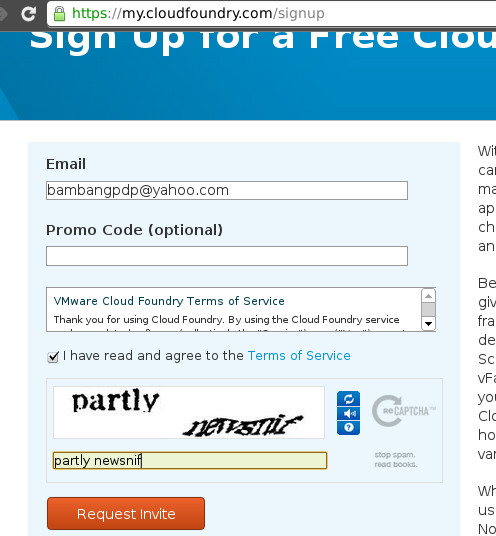
\includegraphics[scale=0.5]{images/cf-signup.jpg}
    \end{center}
    \caption{Pendaftaran di CF}
    \label{fig:cfsignup}
  \end{figure}

Setelah itu, CF akan mengirimkan pemberitahuan bahwa proses pendaftaran selesai seperti di Gambar~\ref{fig:cfsignuphasil}. \textit{Credentials} atau informasi tentang akun kita di CF akan dikirimkan ke e-mail kita seperti pada Gambar~\ref{fig:cfsignupapproved}.
 
  \begin{figure}
    \begin{center}
      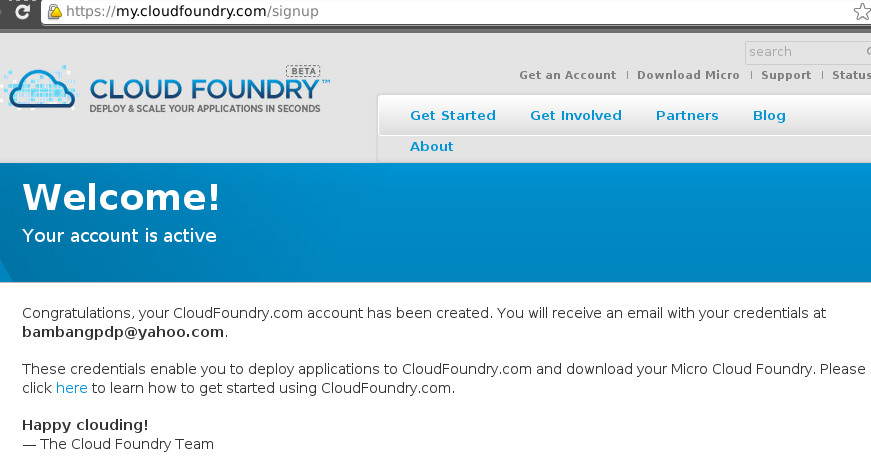
\includegraphics[scale=0.5]{images/cf-signup-hasil.jpg}
    \end{center}
    \caption{Hasil proses pendaftaran di CF}
    \label{fig:cfsignuphasil}
  \end{figure}

  \begin{figure}[t]
    \begin{center}
      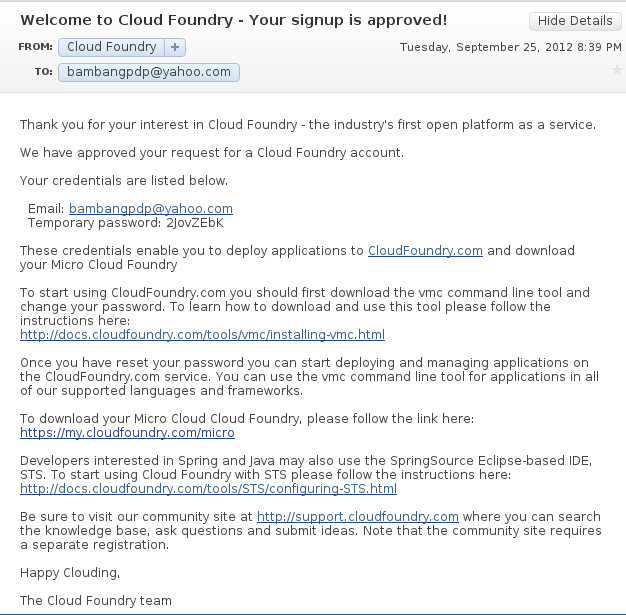
\includegraphics[scale=0.5]{images/cf-signup-approved.jpg}
    \end{center}
    \caption{E-mail persetujuan dan pemberitahuan \textit{credentials}}
    \label{fig:cfsignupapproved}
  \end{figure}

\subsection{Instalasi \textit{Command Line Utilities}}

\index{CloudFoundry!vmc}\textit{Command Line Utilities / CLU)} adalah software yang dijalankan melalui shell / \textit{command line / command prompt}. CLU untuk CF ini dibuat dengan menggunakan Ruby dan didistribusikan dalam bentuk \textit{gem} sehingga untuk instalasi ini diperlukan ruby dan rubygem. Berikut adalah perintah untuk instalasi vmc (CLU dari CF).

\lstset{language=bash,caption=Instalasi vmc}
\begin{lstlisting}
$ gem search vmc --remote | grep "\bvmc\s" 
vmc (0.4.7) 
$ gem install vmc 
Fetching: json_pure-1.6.7.gem (100%)
Fetching: interact-0.5.1.gem (100%)
Fetching: multipart-post-1.1.5.gem (100%)
Fetching: multi_json-1.4.0.gem (100%)
Fetching: rubyzip-0.9.9.gem (100%)
Fetching: cfoundry-0.4.17.gem (100%)
Fetching: clouseau-0.0.2.gem (100%)
Fetching: mothership-0.3.5.gem (100%)
Fetching: manifests-vmc-plugin-0.4.19.gem (100%)
Fetching: tunnel-dummy-vmc-plugin-0.0.2.gem (100%)
Fetching: vmc-0.4.7.gem (100%)
Successfully installed json_pure-1.6.7
Successfully installed interact-0.5.1
Successfully installed multipart-post-1.1.5
Successfully installed multi_json-1.4.0
Successfully installed rubyzip-0.9.9
Successfully installed cfoundry-0.4.17
Successfully installed clouseau-0.0.2
Successfully installed mothership-0.3.5
Successfully installed manifests-vmc-plugin-0.4.19
Successfully installed tunnel-dummy-vmc-plugin-0.0.2
Successfully installed vmc-0.4.7
11 gems installed
Installing ri documentation for json_pure-1.6.7...
Installing ri documentation for interact-0.5.1...
Installing ri documentation for multipart-post-1.1.5...
Installing ri documentation for multi_json-1.4.0...
Installing ri documentation for rubyzip-0.9.9...
Installing ri documentation for cfoundry-0.4.17...
Installing ri documentation for clouseau-0.0.2...
Installing ri documentation for mothership-0.3.5...
Installing ri documentation for manifests-vmc-plugin-0.4.19...
Installing ri documentation for tunnel-dummy-vmc-plugin-0.0.2...
Installing ri documentation for vmc-0.4.7...
Installing RDoc documentation for json_pure-1.6.7...
Installing RDoc documentation for interact-0.5.1...
Installing RDoc documentation for multipart-post-1.1.5...
Installing RDoc documentation for multi_json-1.4.0...
Installing RDoc documentation for rubyzip-0.9.9...
Installing RDoc documentation for cfoundry-0.4.17...
Installing RDoc documentation for clouseau-0.0.2...
Installing RDoc documentation for mothership-0.3.5...
Installing RDoc documentation for manifests-vmc-plugin-0.4.19...
Installing RDoc documentation for tunnel-dummy-vmc-plugin-0.0.2...
Installing RDoc documentation for vmc-0.4.7...
$
\end{lstlisting}

Hasil dari instalasi tersebut adalah sebagai berikut:

\lstset{language=bash,caption=Hasil gem yang terinstall}
\begin{lstlisting}
$ gem list 

*** LOCAL GEMS ***

bigdecimal (1.1.0)
cfoundry (0.4.17)
clouseau (0.0.2)
interact (0.5.1)
io-console (0.3)
json (1.5.4)
json_pure (1.6.7)
manifests-vmc-plugin (0.4.19)
minitest (2.5.1)
mothership (0.3.5)
multi_json (1.4.0)
multipart-post (1.1.5)
rake (0.9.2.2)
rdoc (3.9.4)
rubyzip (0.9.9)
tunnel-dummy-vmc-plugin (0.0.2)
vmc (0.4.7)
$ 
\end{lstlisting}

Setelah itu, tambahkan baris berikut di \textit{\$HOME/.bashrc} (catatan: "/home/bpdp/" adalah direktori \$HOME saya, silahkan sesuaikan dengan tempat anda):

\lstset{language=bash,caption=Mengaktifkan direktori "bin" hasil instalasi gem}
\begin{lstlisting}
export PATH=$PATH:/home/bpdp/.gem/ruby/1.9.1/bin
\end{lstlisting}

Periksa dengan menjalankan opsi help dari vmc:

\lstset{language=bash,caption=Hasil opsi help dari vmc}
\begin{lstlisting}
$ vmc help 
Showing basic command set. Pass --all to list all commands.

Getting Started
  login [USERNAME]	Authenticate with the target
  target [URL]    	Set or display the target cloud, organization, and space
  logout          	Log out from the target
  info            	Display information on the current target, user, etc.

Applications
  apps     	List your applications
  app [APP]	Show app information

  Management
    start APPS...  	Start an application
    delete APPS... 	Delete an application
    push [NAME]    	Push an application, syncing changes if it exists
    stop APPS...   	Stop an application
    restart APPS...	Stop and start an application

Services
  service INSTANCE	Show service instance information
  services        	List your service instances

  Management
    create-service [SERVICE] [NAME]	Create a service
    bind-service SERVICE APP       	Bind a service to an application
    unbind-service SERVICE APP     	Unbind a service from an application
    delete-service [INSTANCE]      	Delete a service
    tunnel [INSTANCE] [CLIENT]     	Tells you to install tunnel-vmc-plugin

Organizations
  create-org [NAME]        	Create an organization
  orgs                     	List available organizations
  delete-org [ORGANIZATION]	Delete an organization
  org [ORGANIZATION]       	Show organization information

Spaces
  create-space [NAME] [ORGANIZATION]	Create a space in an organization
  space [SPACE]                     	Show space information
  delete-space SPACES...            	Delete a space and its contents
  spaces [ORGANIZATION]             	List spaces in an organization

Routes
  create-route [URL]  	Create a route
  delete-route [ROUTE]	Delete a route
  routes              	List routes in a space

Domains
  create-domain NAME    	Create a domain
  delete-domain [DOMAIN]	Delete a domain
  add-domain NAME       	Add a domain to a space
  remove-domain [DOMAIN]	Remove a domain from a space
  domains [SPACE]       	List domains in a space

Options:
      --[no-]color       Use colorful output
      --[no-]script      Shortcut for --quiet and --force
  -V, --verbose          Print extra information
  -f, --[no-]force       Skip interaction when possible
  -h, --help             Show command usage & instructions
  -m, --manifest FILE    Path to manifest file to use
  -q, --[no-]quiet       Simplify output format
  -t, --trace            Show API requests and responses
  -u, --proxy EMAIL      Act as another user (admin only)
  -v, --version          Print version number
$ 
\end{lstlisting}

\subsection{Konfigurasi di Server Cloud}

Pada dasarnya, yang diperlukan hanyalah mengubah target ke server cloud dari CF dan kemudian mengubah password.

\lstset{language=bash,caption=Mengubah target server - belum ada konfigurasi}
\begin{lstlisting}
$ vmc target 
Errno::ENOENT: No such file or directory - /home/bpdp/.vmc/target
For more information, see ~/.vmc/crash
$
\end{lstlisting}

Error di atas terjadi karena file konfigurasi belum dibuat. File konfigurasi tersimpan di direktori \$HOME/.vmc. Mengubah target dilakukan dengan membuat file \textit{target} di direktori tersebut. Isi dari file target tersebut adalah server CloudFoundry, yaitu \textit{https://api.cloudfoundry.com}. Setelah itu, jika dieksekusi lagi, hasilnya adalah sebagai berikut:

\lstset{language=bash,caption=Mengubah target server - setelah konfigurasi}
\begin{lstlisting}
$ vmc target 
 
target: https://api.cloudfoundry.com

$ 
\end{lstlisting}

Setelah itu, setiap kali kita akan melakukan berbagai proses yang melibatkan server ini, kita harus melakukan proses login terlebih dahulu:

\lstset{language=bash,caption=Login ke server}
\begin{lstlisting}
$ vmc login 
target: https://api.cloudfoundry.com

Email> bambangpdp@yahoo.com

Password> ***************

Authenticating... OK

$ vmc info --all
Getting runtimes... OK
Getting frameworks... OK
Getting services... OK

VMware's Cloud Application Platform

target: https://api.cloudfoundry.com
  version: 0.999
  support: http://support.cloudfoundry.com

user: bambangpdp@yahoo.com

runtime   description
java      1.6.0_24   
java7     1.7.0_04   
node      0.4.12     
node06    0.6.8      
node08    0.8.2      
ruby18    1.8.7p357  
ruby19    1.9.2p180  

framework    description
grails       
java_web     
lift         
node         
play         
rack         
rails3       
sinatra      
spring       
standalone   

service      version   provider   description                          
mongodb      2.0       core       MongoDB NoSQL store                  
mysql        5.1       core       MySQL database service               
postgresql   9.0       core       PostgreSQL database service (vFabric)
rabbitmq     2.4       core       RabbitMQ message queue               
redis        2.4       core       Redis key-value store service        
redis        2.2       core       Redis key-value store service        
redis        2.6       core       Redis key-value store service    

$ 
\end{lstlisting}

Untuk mengubah password:

\lstset{language=bash,caption=Mengubah password server}
\begin{lstlisting}
$ vmc passwd 
New Password> **************

Verify Password> **************

Changing password... OK
$
\end{lstlisting}

\subsection{Instalasi dan Konfigurasi Node.js di Komputer Lokal}

Node.js tersedia untuk Linux, Windows, Mac OS X, serta SunOS. Untuk versi Linux, kebanyakan distro sudah menyertakan paket Node.js, hanya saja ada banyak versi dari Node.js dan jika kita menggunakan manajemen paket dari distro Linux, kita hanya bisa menginstall 1 versi saja. Sebagai contoh, di Arch Linux, paket Node.js bisa diinstrall dengan perintah ``pacman -S nodejs'' tetapi hanya pada versi resmi di repo Arch Linux (versi 0.8.16 pada tanggal 7 Januari 2012). 

Langkah instalasi berikut ini adalah langkah untuk instalasi tanpa manajemen paket dari distro Linux.
\begin{itemize}
  \item Ambil paket \textit{binary executable} dari \url{http://nodejs/download} atau langsung ke \url{http://nodejs.org/dist/}. Versi yang digunakan disini adalah 0.8.16. Download file tersebut, kemudian simpan di direktori tertentu (terserah anda, dibuku ini diletakkan di \$HOME/master/nodejs).

\lstset{language=bash,caption=Hasil dari download Node.js}
\begin{lstlisting}
$ ls -la
...
...
-rw-r--r--  1 bpdp users 4406113 Dec 13 06:16 node-v0.8.16-linux-x86.tar.gz
...
...
$ 
\end{lstlisting}

  \item Ekstrak ke direktori yang diinginkan. Node.js akan diinstall di direktori \$HOME/software:

\lstset{language=bash,caption=Ekstraksi Node.js}
\begin{lstlisting}
$ cd 
$ cd software
$ tar -xzvf ~/master/nodejs/node-v0.8.16-linux-x86.tar.gz
$ ln -s node-v0.8.16-linux-x86 nodejs
$ ls -la
....
....
lrwxrwxrwx   1 bpdp users    22 Dec 14 23:45 nodejs -> node-v0.8.16-linux-x86
drwxr-xr-x   6 bpdp users  4096 Dec 13 06:16 node-v0.8.16-linux-x86
....
....
$ 
\end{lstlisting}

  \item Konfigurasi variabel lingkungan. Sebaiknya disimpan pada suatu file (pada buku ini, konfigurasi akan disimpan di \textit{\$HOME/environment/nodejs}):

\lstset{language=bash,caption=Konfigurasi variabel lingkungan Node.js}
\begin{lstlisting}
NODEJS_HOME=/home/bpdp/software/nodejs
 
PATH=$PATH:$NODEJS_HOME/bin
MANPATH=$MANPATH:$NODEJS_HOME/share/man
LD_LIBRARY_PATH=$LD_LIBRARY_PATH:$NODEJS_HOME/lib
C_INCLUDE_PATH=$C_INCLUDE_PATH:$NODEJS_HOME/include
CPLUS_INCLUDE_PATH=$CPLUS_INCLUDE_PATH:$NODEJS_HOME/include
 
export PATH
export MANPATH
export LD_LIBRARY_PATH
export C_INCLUDE_PATH
export CPLUS_INCLUDE_PATH
\end{lstlisting}

  \item Setiap akan menggunakan Node.js, yang diperlukan adalah men-source file konfigurasi tersebut: \textbf{source \~/environment/nodejs}.
\end{itemize}

\section{Pengelolaan Aplikasi di Cloud}

Aplikasi yang dibuat nantinya akan di-deploy ke server CF. Pada umumnya, developer akan melakukan proses untuk upload (\textit{push}), menghapus (\textit{delete}), serta memperbaharui (\textit{update}) aplikasi di server. Jika belum memahami sintaksis JavaScript serta penggunaan npm, jangan kuatir. Tujuan dari bab ini hanya mengenalkan pengelolaan aplikasi di Cloud. Aspek lainnya akan dibahas di bab-bab berikutnya.

\subsection{\textit{Push, Delete, Update} Aplikasi}

Pada pembahasan ini, akan diberikan contoh menggunakan dua kategori, yaitu dengan menggunakan \textit{framework} (ExpressJS - \url{http://expressjs.com}) serta tanpa menggunakan \textit{framework}.

\subsection{Menggunakan Framework ExpressJS}

\lstset{language=bash,caption=Instalasi ExpressJS menggunakan npm}
\begin{lstlisting}
$ npm install -g express
\end{lstlisting}

Jika berhasil, maka kita bisa menggunakan perintah \textit{express} untuk membuat rerangka aplikasi. Sintaksis penggunaan ExpressJS adalah sebagai berikut:

\lstset{language=bash,caption=Perintah express}
\begin{lstlisting}
$ express --help

  Usage: express [options]

  Options:

    -h, --help          output usage information
    -V, --version       output the version number
    -s, --sessions      add session support
    -e, --ejs           add ejs engine support (defaults to jade)
    -J, --jshtml        add jshtml engine support (defaults to jade)
    -H, --hogan         add hogan.js engine support
    -c, --css <engine>  add stylesheet <engine> support (less|stylus) (defaults to plain css)
    -f, --force         force on non-empty directory

$
\end{lstlisting}

Setelah itu, kita bisa membuat rerangka aplikasi ExpressJS dengan cara berikut:

\lstset{language=bash,caption=Menggunakan express untuk membuat rerangka aplikasi}
\begin{lstlisting}
$ mkdir hello 
$ cd hello
$ express 

   create : .
   create : ./package.json
   create : ./app.js
   create : ./public
   create : ./public/images
   create : ./routes
   create : ./routes/index.js
   create : ./routes/user.js
   create : ./public/stylesheets
   create : ./public/stylesheets/style.css
   create : ./views
   create : ./views/layout.jade
   create : ./views/index.jade
   create : ./public/javascripts

   install dependencies:
     $ cd . && npm install

   run the app:
     $ node app

$
\end{lstlisting}

Pada rerangka aplikasi tersebut, terdapat file \textit{package.json} untuk mendefinisikan aplikasi serta dependensi-nya dan app.js yang merupakan file utama untuk dijalankan pada server.

\lstset{language=Javascript,caption=package.json untuk ExpressJS}
\begin{lstlisting}
{ 
  "name": "hello-node", 
  "version": "0.0.1", 
	"private": true,
	"scripts": {
		"start": "node app"
	},
  "dependencies":{ 
    "express": "3.0.6".
		"jade": "*"
  } 
} 
\end{lstlisting}

\lstset{language=Javascript,caption=app.js untuk ExpressJS}
\begin{lstlisting}
/**
 * Module dependencies.
 */

var express = require('express')
  , routes = require('./routes')
  , user = require('./routes/user')
  , http = require('http')
  , path = require('path');

var app = express();

app.configure(function(){
  app.set('port', process.env.PORT || 3000);
  app.set('views', __dirname + '/views');
  app.set('view engine', 'jade');
  app.use(express.favicon());
  app.use(express.logger('dev'));
  app.use(express.bodyParser());
  app.use(express.methodOverride());
  app.use(app.router);
  app.use(express.static(path.join(__dirname, 'public')));
});

app.configure('development', function(){
  app.use(express.errorHandler());
});

app.get('/', routes.index);
app.get('/users', user.list);

http.createServer(app).listen(app.get('port'), function(){
  console.log("Express server listening on port " + app.get('port'));
});
\end{lstlisting}

Edit file \textit{routes/index.js} sebagai berikut:

\lstset{language=Javascript,caption=Hasil edit routes/index.js}
\begin{lstlisting}
/*
 * GET home page.
 */

exports.index = function(req, res){
  res.render('index', { title: 'Express app at CloudFoundry' });
};
\end{lstlisting}

Setelah itu, install modul-modul yang diperlukan dengan perintah \textit{npm install} pada direktori tersebut. npm akan membaca file package.json kemudian menginstall modul-modul sesuai dengan deskripsi pada \textit{dependencies}. Setelah diuji pada komputer lokal dengan perintah \textit{node app}, dan sukses bisa diakses di browser dengan alamat \textit{http://localhost:3000}, maka aplikasi tersebut bisa di-deploy di CloudFoundry. Proses deployment digambarkan sebagai berikut (anda sudah harus login menggunakan perintah \textit{vmc login} sebelumnya) dan berada di direktori tempat aplikasi tersebut berada:

\lstset{language=bash,caption=Deployment aplikasi ExpressJS ke CF}
\begin{lstlisting}
$ vmc push
Name> hello-express

Instances> 1

1: node
2: other
Framework> node

1: node
2: node06
3: node08
4: other
Runtime> 3

1: 64M
2: 128M
3: 256M
4: 512M
5: 1G
Memory Limit> 64M

Creating hello-express... OK

1: hello-express.cloudfoundry.com
2: none
URL> hello-express.cloudfoundry.com

Updating hello-express... FAILED
The URI: "hello-express.cloudfoundry.com" has already been taken or reserved

1: hello-express.cloudfoundry.com
2: none
URL> bpdp-hello-express.cloudfoundry.com

Updating hello-express... OK

Create services for application?> n

Save configuration?> n

Uploading hello-express... OK
Starting hello-express... OK
Checking hello-express... OK

$ 
\end{lstlisting}

Hasilnya terlihat pada tampilan browser di Gambar~\ref{fig:modul1-hello}

  \begin{figure}
    \begin{center}
      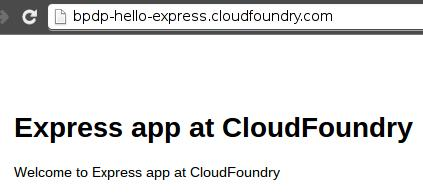
\includegraphics[scale=0.5]{images/bpdp-hello-express.jpg}
    \end{center}
    \caption{Hasil push ke server}
    \label{fig:modul1-hello}
  \end{figure}

Aplikasi yang sudah dibuat seringkali diubah, oleh karena itu vmc juga menyediakan fasilitas untuk Mengupdate aplikasi. 

\lstset{language=Javascript,caption=Update: menambahkan versi Node.js ke routes/index.js}
\begin{lstlisting}
/*
 * GET home page.
 */

exports.index = function(req, res){
	var nv = process.version;
  res.render('index', { title: 'Express app at CloudFoundry with Node.js ' + nv });
};
\end{lstlisting}

\lstset{language=bash,caption=Mengupdate aplikasi di server}
\begin{lstlisting}
$ vmc apps
Getting applications... OK

name              status    usage     runtime   url                                      
hello-express     running   1 x 64M   node08    bpdp-hello-express.cloudfoundry.com      
$ vmc push hello-express
Uploading hello-express... OK
Stopping hello-express... OK

Starting hello-express... OK
Checking hello-express... OK
$ 
\end{lstlisting}

Hasilnya bisa dilihat di Gambar~\ref{fig:modul1-hello-update}

  \begin{figure}
    \begin{center}
      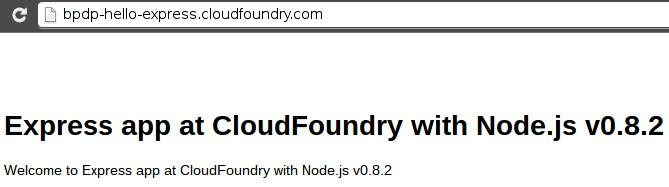
\includegraphics[scale=0.5]{images/bpdp-hello-express-update.jpg}
    \end{center}
    \caption{Hasil update dengan menyertakan versi Node.js}
    \label{fig:modul1-hello-update}
  \end{figure}

Untuk menghapus aplikasi:

\lstset{language=bash,caption=Menghapus aplikasi yang di-deploy di CF}
\begin{lstlisting}
$ vmc delete bpdp-m1-hellonoframework
Really delete bpdp-m1-hellonoframework?> y

Deleting bpdp-m1-hellonoframework... OK

$ 
\end{lstlisting}

Pada saat deployment, kita juga bisa memilih versi Node.js (runtime) sebagai berikut:

\lstset{language=bash,caption=Deployment ke CF dengan memilih runtime Node.js}
\begin{lstlisting}
$ vmc push --runtime=node08 
Name> bpdp-hello-express06

Instances> 1

1: node
2: other
Framework> node

1: 64M
2: 128M
3: 256M
4: 512M
5: 1G
Memory Limit> 64M

Creating bpdp-hello-express06... OK

1: bpdp-hello-express06.cloudfoundry.com
2: none
URL> bpdp-hello-express06.cloudfoundry.com

Updating bpdp-hello-express06... OK

Create services for application?> n

Save configuration?> n

Uploading bpdp-hello-express06... OK
Starting bpdp-hello-express06... OK
Checking bpdp-hello-express06... OK
$
\end{lstlisting}

Hasilnya bisa dilihat di Gambar~\ref{fig:modul1-hello-ganti-runtime}

  \begin{figure}
    \begin{center}
      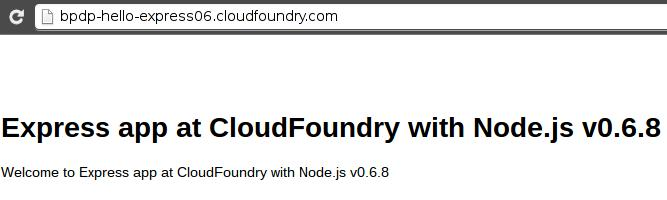
\includegraphics[scale=0.5]{images/bpdp-express-hello-update06.jpg}
    \end{center}
    \caption{Deployement menggunakan versi runtime tertentu}
    \label{fig:modul1-hello-ganti-runtime}
  \end{figure}

\subsection{Tanpa Framework}

Tanpa \textit{framework}, yang kita perlukan hanyalah langsung mem-\textit{push} file yang kita buat (dalam contoh ini adalah app.js):

\lstset{language=Javascript,caption=app.js tanpa framework}
\begin{lstlisting}

var http = require('http'); 
var url = require("url"); 

http.createServer(function (req, res) { 

    var pathname = url.parse(req.url).pathname; 

    res.writeHead(200, {'Content-Type': 'text/html'}); 
    res.write("Hello NodeJS <u>" + process.version + "</u>"); 
    res.write("<br />Request for <b>" + pathname + "</b> received."); 
    res.end(); 

}).listen(1337);
\end{lstlisting}

Proses deployement adalah sebagai berikut:

\lstset{language=bash,caption=Deployment app.js tanpa framework}
\begin{lstlisting}
$ vmc push
Name> hello-noframework

Instances> 1

1: node
2: other
Framework> node

1: node
2: node06
3: node08
4: other
Runtime> 3

1: 64M
2: 128M
3: 256M
4: 512M
5: 1G
Memory Limit> 64M

Creating hello-noframework... OK

1: hello-noframework.cloudfoundry.com
2: none
URL> hello-noframework.cloudfoundry.com

Updating hello-noframework... OK

Create services for application?> n

Save configuration?> n

Uploading hello-noframework... OK
Starting hello-noframework... OK
Checking hello-noframework... OK
$
\end{lstlisting}

Hasilnya bisa dilihat pada Gambar~\ref{fig:modul1-hello-no-framework}

  \begin{figure}
    \begin{center}
      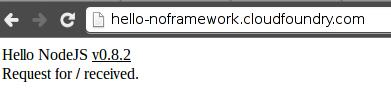
\includegraphics[scale=0.5]{images/hello-noframework.jpg}
    \end{center}
    \caption{Hasil deployement app.js tanpa framework}
    \label{fig:modul1-hello-no-framework}
  \end{figure}
